%  SingleXBs
%  Created by Dave Williams on 2009-06-25.
%  

% header (fold)
\documentclass[]{article}

\usepackage{setspace, float, fancyhdr}
\usepackage[pdftex]{graphicx}
\usepackage[utf8]{inputenc}
\usepackage[round,numbers,sort&compress]{natbib} 
\addtolength{\parskip}{\baselineskip}
\setlength{\parindent}{0in}

% Multipart figures
%\usepackage{subfigure}
% Package for including code in the document
%\usepackage{listings}

\title{Simple and complex multidimensional actomyosin crossbridges}
\author{C Dave, Mikey R, Tommy D}
\date{2009 - 06 - 25}
% header (end)

\begin{document}

\maketitle

\begin{abstract} 
\marginpar{Currently, abstract gives main points of the paper.}
The 4 spring crossbridge (4sXB) is able to accurately model the movements believed to be behind the generation of force by myosin during the power stroke.
The 2 spring crossbridge (2sXB) shares many of the desirable properties of the 4sXB, such as the elimination of linear offsets in favor of experimentally measured changes in lever angle.
Both the 4sXB and the 2sXB maintain similar kinetics to previous work at resting lattice spacings, permitting more direct comparison of work done with either system to previous studies.
Unlike the 4sXB, the length and angle of the springs comprising the 2sXB can be analytically determined for any chosen head position without the use of iterative techniques.
Both the 4sXB and the 2sXB are able to measure the radial forces generated by during the production of axial force.
Similarly, both proposed crossbridge systems take lattice spacing into account in every aspect of their operation.
Lattice spacing dependent kinetics are derived based on the work of Pate and Cooke.
Lattice spacing dependent axial and radial forces are measured and considered.
\end{abstract}

Keywords: myosin; spatially-explicit model; crossbridge kinetics

\paragraph*{Author Summary} % (fold)
Models of muscle contraction have long treated the molecular motor myosin as a simple spring oriented parallel to its direction of movement. 
This does not allow for the investigation of phenomena such as the perpendicular force observed during shortening, or the dependence of the maximum force produced on spacing between the contractile filaments that comprise muscle.
We demonstrate an alternative model, computationally simple enough to use in large networked models, that incorporate both linear and torsional or angular springs. These models capture much of the behavior missing from previous efforts.
% paragraph author_summary (end)

\section{Introduction} %(fold)

% * Set out view of force generation and power stroke
% * Mismatch with single spring crossbridge
%  - Considerations in modeling (computational complexity) 
% Needs more, come back to this

\textbf{Needs a purpose. Get results done and rewrite}

Sarcomere-scale modeling of muscle contraction has largely changed since the introduction of the sliding crossbridge model in the 1950s, but the geometry of the individual crossbridges used has remained largely unaltered. 
While thermodynamic account had been introduced to the crossbridge kinetics, compliance has been introduced to the filaments, and multiple filaments have been arranged to mimic the lattice, the one dimensional single spring nature of the crossbridge has continued to be used as a model of the mechanism of force generation.

The now-traditional single spring crossbridge introduced by \citet{Huxley:1957:p255} has been the dominant model used in modeling studies since its introduction. 
The geometry of the single spring crossbridge has remained largely unchanged while the kinetics underlying transitions between force generating states have been increased in complexity throughout subsequent work. \citep{Pate:1989:p181, Daniel:1998:p1611, Chase:2004:p204, Tanner:2007:pe115}

\citet{Houdusse:2001:p182} and others have proposed that the region of the lever arm directly adjacent to the converter region is a flexible area that acts as a spring. This pliant region is the most likely candidate for the job of torsional spring. 


% section introduction (end)


\section{Materials and Methods}  % (fold)

 % * Overview
 %  - Classes of crossbridges: 1, 4, and 2 springs
 % * Geometry
 %  - Spring configurations
 %   = Single spring axially parallel
 %   = Four spring correspondence to physical parts
 %   = Sources of four spring values
 %   = Acknowledge powerstroke distance
 %   = Two spring fit to replicate four spring
 %  - Force generated via displacement
 %  - Calculation of spring lengths/angles
 % * Kinetics
 %  - Free energy in each state
 %   = Liberation of energy by Pi hydrolysis
 %  - Calculation of binding rate
 %   = Perturbation of crossbridge head
 %   = Probability of binding based on distance to binding site
 %  - Powerstroke rate
 %   = Distortion dependence
 %  - Unbinding rate
 %  - Calculation of reverse rates

We restrict our analysis to representations of crossbridges that are useful for spatially explicit modeling of the half-sarcomere, i.e.\ models utilizing from one to several springs.
Representations of the crossbridge as a single spring have been used extensively in previous work and serve as a baseline against which we can compare more complicated models.
A crossbridge comprised of four springs is able to replicate both the known geometry of the crossbridge and the movements that comprise the power stroke.
A simpler crossbridge consisting of just two springs, able to replicate most of the four spring crossbridge's behavior, is also described.

\subsection*{Geometry} % (fold)

\paragraph{Spring configurations} % (fold)
The 1sXB consists of a single linear spring aligned parallel to the thick and thin filaments.
As described above, it is insensitive to changes in lattice spacing and is unable to account for radial forces generated during axial shortening.

The 4sXB uses two linear and two torsional springs to represent the myosin head, as depicted in Fig \ref{fig:types}D.
This allows the springs used in the model to closely correspond to pieces of the crossbridge.
Specifically the four springs correspond to the S2 attachment region, the lever arm, the pliant region/converter domain, and the globular head region.
Additionally, the additional springs of the 4sXB cause it to occupy two dimensions, where the 1sXB only occupies one.
This two dimensionality allows the 4sXB to be embedded in a space that takes the distance between thick and thin filaments into account, introducing lattice spacing dependence.

The 2sXB uses one linear and one torsional spring to represent the myosin head, as depicted in Figure~\ref{fig:types}C.
This crossbridge acts as a simplification of the 4sXB, retaining movement generated by a lever arm, but altering the length of the lever such that it can bridge the entire distance between the thick and thin filaments.
The parameters characterizing the 2sXB are chosen to match the step size and kinetics of the 2sXB to those of the 4sXB.

Each type of crossbridge has several physical parameters that must be set before they may be used.
Each linear spring (one in the 1sXB, two in the 4sXB and one in the 2sXB) requires a rest length and spring constant, while each torsional spring (two in the 4sXB and one in the 2sXB) requires a rest angle and spring constant.
The rest length or angle of one spring in each crossbridge is altered during the transition from a weakly bound state to a strongly bound state, in order to produce the force that tensions the linked filaments.

% MORE SHOULD BE ADDED ON PARAMETER CHOICE HERE

% paragraph spring_configurations (end)

\paragraph{Displacement and force generation} % (fold)
The geometry of the 1sXB model of the crossbridge has evolved with an eye towards accounting for the offset generated by the powerstroke and the energy utilized in the creation of this offset. 
From these two concerns the force the spring (assuming it to be a linear one) can produce is accounted for. 
In a two dimensional model there is the additional goal of replicating the crossbridge's sensitivity to lattice spacing and multidimensional force generated. 
% paragraph displacement_and_force_generation (end)

\paragraph{Calculation of spring lengths and angles} % (fold)
When the 1sXB is distorted such that the myosin head is horizontally offset from thick filament attachment site relative to its resting position, the length of the 1sXB's spring is simple to find as it must completely span the head to thick filament attachment distance.
The lengths and angles of the springs in the 2sXB and 4sXB must take into account the radial distance they must cover as well, but remain simple to calculate.
The 2sXB may be analytically determined, as it has all spring values set by the choice of a head location, with arm length and angle given by $r(h_x, h_y)=(h_x^2 + h_y^2)^{1/2}$ and $\theta(h_x, h_y)=\arctan(h_y/h_x)$, respectively.
The 4sXB suffers from increased computational complexity over the 1sXB and 2sXB systems in that iterative optimization is required to find the location of the distal torsional spring representing the converter region when the crossbridge's head is moved to a new location.
We use a modification of Powell's ``dog-leg'' method\footnote{Present in the SciPy package of computational tools.} to relax the location of the distal torsional spring to that which results in the lowest energy state of the 4sXB.
Once the distal torsional spring's location is known (as $(c_x, c_y)$), the angle of the proximal torsional spring and the lengths of the two linear springs are analytically determinable.
The angle of the proximal torsional spring is given as $\phi(c_x, c_y)=\arctan(c_y/c_x)$, the length of the proximal linear spring as $\ell(c_x, c_y)=(c_x^2 + c_y^2)^{1/2}$, the angle of the distal torsional spring as $\theta(c_x, c_y, h_x, h_y) = \arctan((h_y-c_y)/(h_x-c_x)) + \pi - \phi(c_x, c_y)$, and the length of the distal linear spring as $r(c_x, c_y, h_x, h_y)=((h_x-c_x)^2 + (h_y-c_y)^2)$.
% paragraph calculation_of_spring_lengths_and_angles (end)
% subsection geometry (end)

\subsection*{Kinetics} % (fold)
% * Kinetics
%  - Three states
%  - Distorsion sensitive
%  - Free energy in each state
%   = Liberation of energy by Pi hydrolysis
%  - Calculation of binding rate
%   = Perturbation of crossbridge head
%   = Probability of binding based on distance to binding site
%  - Powerstroke rate
%   = Distortion dependence
%  - Unbinding rate
%  - Calculation of reverse rates
As in other recent works, such as \citet{Tanner:2007:pe115}, we choose to use a simplified three state model of the crossbridge cycle with energies based on the work of Pate and Cooke in \citet{Pate:1989:p181}. 
This simplified system allows for the most direct linking of the crossbridge's kinetics and chemo-mechanics; the three kinetic states being directly comparable to the myosin configurations described in \citet{Houdusse:2000:p11238}.
A secondary benefit of a three state kinetics system is that it allows multiple-motor models which use our many-spring crossbridges to more easily compare their results to those from the aforementioned previous models.

The three states represented in our kinetics are an unbound state, a loosely-bound state, and a tightly-bound force-generating state.
As depicted in figure \ref{fig:types} A, these states correspond to a Myosin-ADP-Pi state, an Actin-Myosin-ADP-Pi state, and an Actin-Myosin-ADP state.

The kinetics of both the two spring and the four spring models are strain dependent and are essentially transforms of the free energy landscapes experienced by the crossbridges in their different states.
These free energies are a function of the distortion necessary to move the point representing the crossbridge's head to the point where we presume a binding site to be.
Examples of these free energy landscapes are visible in figures \ref{fig:2s}A and \ref{fig:4s}A, with cuts through them at multiple lattice spacings visible in figures \ref{fig:2s}B and \ref{fig:4s}B.

The binding of both the two and four spring crossbridges is determined by Monte-Carlo simulation of their diffusion as a result of being perturbed by Boltzmann derived energy distributions. 
After a new head location is found, a binding probability is calculated that decreases exponentially with distance from the potential binding site. 
This probability is tested against a random number from a uniform distribution to determine if binding occurs.

\paragraph{Free energy in each state} % (fold)
The total energy, liberated by the hydrolysis of a $P_i$, available to a crossbridge is dependent on the concentrations of $ATP$, $ADP$ and $P_i$ in the system and is given by $\Delta G = -\Delta G_{0,ATP} - \ln \frac{[ATP]}{[ADP] [P_i]}$. 
In the weakly bound and strongly bound states a portion of that energy has been made available to the crossbridge, allowing the crossbridge in the latter two states to convert at most 28\% or 68\% of $\Delta G$ into useable work respectively. \citep{Pate:1989:p181, Tanner:2007:pe115}
These efficiency factors are used as $\alpha=0.28$ and $\eta=0.68$ below.
The free energy of a crossbridge in each state it a function of both the energy available as described above and the strain that the crossbridge is currently experiencing as a result of post-binding distortion.
Combining the distortion dependence and liberated energy terms gives us the total free energy of the crossbridge in each state.
The free energy of the 4sXB system in each state is: 
%Energy of the four spring crossbridge
\begin{eqnarray}
\label{4sEnergy}
U_1(\phi,\ell,\theta,r) & = & 0 \nonumber \\
U_2(\phi,\ell,\theta,r) & = & \alpha \Delta G + \frac{k_\phi (\phi-\phi_0)^2 + k_\ell (\ell-\ell_0)^2 + k_\theta (\theta-\theta_0)^2 + k_r (r-r_0)^2}{2} \nonumber \\
U_3(\phi,\ell,\theta,r) & = & \eta \Delta G + \frac{k_\phi (\phi-\phi_0)^2 + k_\ell (\ell-\ell_0)^2 + k_\theta (\theta-\theta_1)^2 + k_r (r-r_0)^2}{2} \nonumber
\end{eqnarray}
The free energy of the 2sXB system in each state is: 
% Energy of the two spring crossbridge
\begin{eqnarray}
\label{2sEnergy}
	U_1(r,\theta) & = & 0 \nonumber \\
    U_2(r,\theta) & = & \alpha \Delta G + \frac{k_r (r - r_0)^2 + 
                        k_\theta (\theta - \theta_0)^2}{2} \nonumber \\
    U_3(r,\theta) & = & \eta \Delta G   + \frac{k_r (r - r_1)^2 + 
                        k_\theta (\theta - \theta_1)^2}{2} \nonumber
\end{eqnarray}

% paragraph free_energy_in_each_state(end)

\paragraph{Calculation of binding rate} % (fold)
% Perturbation of crossbridge head
Our binding rates are a determined by thermally forcing unattached heads to a diffused location and then applying a probability of attachment that is an exponential function of the distance from the diffused location to the nearest available actin site.
The thermal forcing of the unattached heads take the form of choosing an offset from a Boltzman distribution for each of the head's constituent springs, finding their resulting lengths and angles, and then using those values to determine the new head location.
The PDF of the an offset location is given by  $P(x) = \sqrt{k / (2 \pi kT)} \exp^{-(k x^2)/(2 kT)}$ where $x$ is the offset, $k$ is the spring constant of the spring in question, and $T$ is the system's temperature.
% Probability of binding based on distance to binding site
Once the offset of each spring is determined, the new head location can be determined from the spring system's geometry and the distance to the binding site found.
Myosin binding is determined to be a exponential function of the distance ($dist$) from the myosin head to the available binding site, such that the probability of the binding is given by $r_{12}(dist) = \gamma \exp ^{dist}$, where $\gamma$ is a scaling factor.
Such a system is very computationally efficient in use, but binding rates as a function of myosin head starting location (as opposed to head to binding stie distance) must be computed by approximation as a fraction of $n$ binding opportunities, using a newly diffused head location and checking against a random number $rand$, ranging from zero to one, which is generated for each trial thus: 
$r_{12} = ( \sum^n ( 1\; \textrm{if}\; \gamma \exp^{-(\textrm{post diffusion distance)}}>rand ,\; \textrm{else}\; 0) )/n$.
This is applied uniformly to the 4sXB and the 2sXB, with the only difference being the number of springs subject to thermal forcing in each instance.
% paragraph calculation_of_binding rate (end)

\paragraph{Powerstroke and detachment rates} % (fold)
% Distortion dependence
The rate of transition from a weakly bound state to a strongly bound one and the rate of detachment from a strongly bound state are distortion dependent and based on the earlier work of \citet{Pate:1989:p181} and \citet{Tanner:2007:pe115}, but generalized to be useable by the 4sXB and 2xB in two-dimensional space. % Recheck Pate&Cooke's work
Distortion dependence is introduced into the $r_{23}$ and $r_{31}$ rates as a term based on the differences in free energy between the current state and the one being considered for transition. 
This means that transitions are more likely when they are energetically favorable and less likely in other circumstances, a natural scheme based in the geometry of the crossbridges.
The particular rates are as follows for both the 4sXB and the 2sXB:
$$r_{23}(U_2, U_3) = 0.001 + 0.5 * (1 + \tanh(0.6 (U_2 - U_3))) $$
$$r_{31}(U_3, U_1) = e^{-1 / (U_3 - U_1)}$$
% paragraph unbinding_rate (end)

\paragraph{Calculation of reverse rates} % (fold)
% Technique of reverse rate calculation
The rates of transitions in the direction opposite from those described above, e.g.\ from strongly to weakly bound or from a weakly bound state to an unbound state, are given by the thermodynamically balancing formula $r_{ij}/r_{ji}=\exp^{U_i-U_j}$ where $r_{ij}$ is the reverse rate and $r_{ji}$ is the forward rate.
For the transition from a weakly bound state to an unbound state this requires that the reverse transition is again treated as a fraction of a sum of $n$ transition opportunities.
% paragraph calculation_of_reverse rates (end)
% subsection kinetics (end)

% section materials_and_methods (end)


\section{Results} % (fold)

 % Results, talking about the figures:
 % Figure 2 shows shift of center of energy profile as lattice spacing changes
 % Shows smaller shift of center of binding probabilitiy
 % Very different rates of power stroke between the two crossbridges
 % Power stroke rates are less depencent on lattice spacing for overall rateas than either other forward rate
 % Four spring detachment rates that still shift in center by as much as 5 nm as lattice spacing changes
 % Detachment rates for the two spring crossbridge that are less dependent on lattice spacing for their center but still very dependent on lattice spacing for their overall rates
 %  * Description of four spring crossbridge kinetics
 %   - Energy bean shapes
 %   - Extension of Pate and Cooke work, may be subsumed in methods
 %  * Comparison of two spring crossbridge to four spring crossbridge
 %   - Closeness of the cuts in Figure 3
 %  * Axial forces generated, varying with lattice spacing
 %  * Radial forces generated & compressive calcs, versus lattice spacing

The obvious and intended consequence of the two and four spring crossbridges is the inclusion of a sensitivity to lattice spacing in the kinetics and force governing and generated by the crossbridge head. 
In addition to scaling the probability of crossbridge interaction with an available binding site, altering the lattice spacing in the two and four spring crossbridges also shifts the offsets of the binding sites that yield optimum probabilities of crossbridge interaction, effectively forward biasing the binding locations at larger lattice spacings.
A radial force component is introduced alongside these other results that expands the possibilities for dual or multi filament models which use this type of crossbridge.

\paragraph{Key points of transition rates and energies vary with lattice spacing} % (fold)
% paragraph key_points_of_transition_rates_and_energies_vary_with_lattice_spacing (end)


\paragraph{Magnitude of transition rates and energies vary with lattice spacing} % (fold)
% paragraph magnitude_of_transition_rates_and_energies_vary_with_lattice_spacing (end)


\paragraph{Kinetics at rest lattice spacings are similar to previous results} % (fold)
% paragraph kinetics_at_rest_lattice_spacings_are_similar_to_previous_results (end)

\paragraph{Radial forces are on same order as axial forces, dependent on lattice spacing and axial offset} % (fold)
% paragraph radial_forces_are_on_same_order_as_axial_forces_dependent_on_lattice_spacing_and_axial_offset (end)

\paragraph{Lattice Spacing Dependence of Kinetics} % (fold)
Figures \ref{fig:2s} and \ref{fig:4s} depict the results of modeling a single crossbridge with two and four springs, respectively.
On the left side of the two figures, the free energies and kinetics of the crossbridges are plotted against various $d_{1,0}$ lattice spacings. 
Changes in lattice spacing here alter the operation of the crossbridge, reflecting the greater or lesser strain that the crossbridge will be subject to when it is stretched to a greater or lesser extent as the filament lattice is compressed or expanded.

On the right sides of figures \ref{fig:2s} and \ref{fig:4s} sequential cuts through the landscape of lattice spacings are taken, in order to better depict the shifting of the probabilities of transition.
These sequential slices depict ...

% paragraph lattice_spacing_dependence_of_kinetics (end)

\paragraph{Forward Biasing of Binding} % (fold)
I am currently unsure as to what should be said about the forward biasing of binding.
Forward biasing of binding, as we have been using it, refers to the elimination of the need for an arbitrary offset being present when the crossbridge is in either of the first two states, but not when it is in the force generating configuration.
This offset of the myosin head can also be thought of as the spring representing the crossbridge head having a different rest length in the unbound state and the loosely bound state than it does in the tightly bound state. 
This offset or altered rest length is what determines the stroke distance of the single spring crossbridge and has been a difficult parameter to pin down as estimates of myosin stroke size have varied from as little as 1 nm to as large as 10 nm (TK:need citation). 
One reason for this large variance may be that assigning a crossbridge step length requires using only one parameter for a movement that is the combination of several smaller and distinct sub-motions.
By treating each of these sub-motions individually, we are able to base the powerstroke of the crossbridge on inputs that can be more accurately determined by examination of existing crystallography structures.
% paragraph forward_biasing_of_binding (end)

\paragraph{Axial and Radial Forces} % (fold)
In addition to the changes to the kinetics at various lattice spacings described above, the axial force generated by the crossbridge is now lattice spacing dependent and there exists a radial force component that was previously absent.
% paragraph axial_and_radial_forces (end)

% section results (end)


\section{Discussion} % (fold)

 % Discussion, integration into the field:
 %  * Provides new crossbridge mechanics for use in models
 %   - Comparison to single spring system
 %   - Low computational requirements of 2s crossbridge
 %   - Possible: balancing radial forces with multiple filaments
 %  * No longer dependent on strained binding, moving towards non-ratchet
 %   - 1s is rectification based as in refs 1,2 of Davis & Epstein 2009
 %   - Both 2s & 4s allow a power stroke mechanism (recalc spring consts)
 %  * Axial forces compared to experimental data
 %   - Comparison Schoenberg work (TNCG/xxCG versus xNxx/xNCx)
 %   - Ask M+T what experimental work would be good to compare to
 %   - Comparison to dextran LS compression and force levels? Probably not.
 %  * Radial forces and experimental observations of compression (Checchi)
 %   - Check magnitude of forces needed

\paragraph{Lattice spacing alters both likelihood of interaction and likely interaction location} % (fold)
% paragraph lattice_spacing_alters_both_likelihood_of_interaction_and_likely_interaction_location (end)


\paragraph{Strain and force generation at the level of a single crossbridge depend on lattice spacing} % (fold)
% paragraph strain_and_force_generation_at_the_level_of_a_single_crossbridge_depend_on_lattice_spacing (end)

\paragraph{Modeled radial forces are too large to ignore} % (fold)
% paragraph modeled_radial_forces_are_too_large_to_ignore (end)

\paragraph{Step size varies with lattice spacing for a two spring crossbridge} % (fold)
Inherent in the geometry of the 2sXB and the 4sXB is a change in step size with a change in lattice spacing.
Step size at a given lattice spacing is defined as the axial distance a myosin head moves between pre- and post-powerstroke angles if unconstrained in the axial direction and allowed to settle into the position which minimizes the energy of the crossbridge.
These changes in step size occur because the angle which a given axial movement subtends increases with decreasing lattice spacings.
This scenario also depends on the linear spring between the myosin's pivot point and the thin filament changing in length to accommodate differing lattice spacings.
The single linear spring of the 2sXB is the only means by which the 2sXB may span the distance from the single torsional spring to the thin filament and thus must change with lattice spacing.
However, the 4sXB is also possessed of the torsional and linear springs which are more proximal to the thick filament.
These additional springs also adjust with lattice spacing, allowing the location of the 4sXB's pivot point to alter so that the difference in step size with changes in lattice spacing is smaller, although still present.
This is yet another factor that may alter the force generated at different lattice spacings, increasing the strain and probability of detachment shortly after completing the powerstroke at larger lattice spacings.
% paragraph step_size_varies_with_lattice_spacing_for_a_two_spring_crossbridge (end)


\paragraph{Comparison to previous systems} % (fold)
This discussion owes a debt to \citet{Schoenberg:1980:p1802} and \citet{Schoenberg:1980:p1627} which contain a proposal and analysis of several different types of crossbridges, primarily two spring crossbridges where the S2 arm is represented as a linear spring and the S2-S1 junction area is represented as a torsional spring. 
This system requires iterative solution methods, as our four spring crossbridge does, but restrains the crossbridge to an area within one S1 length of the line in which the S2 segment is set.
% paragraph comparison_to_previous_systems (end)

% section discussion (end)


\clearpage
\section{Figures} % (fold)

\begin{figure}[htbp]
    \begin{center}
    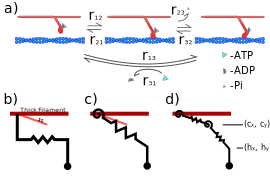
\includegraphics[width=3.2in]{../imgs/Figure1.pdf}
    \label{fig:types}
    \caption{
        \textbf{Kinetic scheme and crossbridge types under investigation.} 
        The three state kinetic system used both here and in prior models is shown in subfigure a). The three states represented are an unbound state (1), a loosely bound state (2), and a strongly bound state (3). The binding rate ($r_{1,2}$), strong transition rate ($r_{2,3}$), and unbinding rate ($r_{3,1}$) at a given location are functions of the energy stored in the springs representing the crossbridge, if the crossbridge head is moved to that location. The reverse rates ($r_{2,1}$, $r_{3,2}$, and $r_{1,3}$) are all functions of the forward transition rates.
        Subfigures b), c), and d) show the various spring based representations of the crossbridge. Subfigure b) shows the single spring crossbridge representation used in models since \protect\cite{Huxley:1957:p255}. Subfigure c) shows the two spring system, consisting of a torsional/angular spring and a linear spring, that we propose to allow the modeling of radial forces. Finally, subfigure d) shows the four spring system using two torsional and two linear springs which we also compare to the single and dual spring crossbridges.
    }
    \end{center}
\end{figure}

\begin{figure}[htbp]
    \begin{center}
    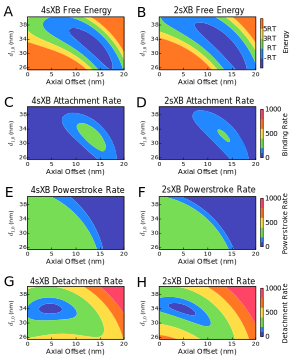
\includegraphics[width=3.2in]{../imgs/Figure2.pdf}
    \label{fig:2s}
    \caption{
        \textbf{Energy and kinetics of the two spring crossbridge with varying axial offsets and lattice spacings.} 
        The free energy of the four spring crossbridge at various lattice spacings (represented along the y-axis), with the head stretched to an axial offset from the point where it attaches to the thick filament (zero on the x-axis) is depicted in a). Simmilarly, the free energy of the two spring crossbridge is represented in b).
        The subfigures c) and d) show $r_{1,2}$, the probability that the four and two spring crossbridges will transition from an unbound state to a bound state, and the dependence of this transition on both the axial offset of the open binding site from the myosin thick filament attachment site and the lattice spacing $d_{1,0}$ which is a function of the distance between the binding site and the thick filament attachment point of the myosin head. Subfigure c) depicts this probability for the four spring crossbridge as a two dimensional contour with the same axes as a) while subfigure d) depicts the transition probabilities for the two spring crossbridge.
        Subfigures e) and f) show $r_{2,3}$, the probability of transition from a weakly bound state to a strongly bound state, for the same crossbridges, with the same axes and scales as c) and d) show $r_{1,2}$.
        Subfigures g) and h) show $r_{3,1}$, the probability of unbinding from a strongly bound state, for the same crossbridges, with the same axes and scales as c) and d) show $r_{1,2}$.
        The reverse rates, $r_{2,1}$, $r_{3,2}$, and $r_{1,3}$ may be back-calculated from the forward rates via the method described in \cite{Tanner:2007:pe115}.
    }
    \end{center}
\end{figure}

\begin{figure}[htbp]
    \begin{center}
    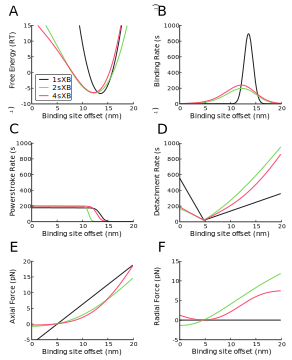
\includegraphics[width=3.2in]{../imgs/Figure3.pdf}
    \label{fig:4s}
    \caption{
        \textbf{Energy and kinetics of the four, two and single spring crossbridges at the resting lattice spacing.}
        Comparison of traditional single spring crossbridge properties to those of the two spring crossbridge at resting lattice spacing.
    }
    \end{center}
\end{figure}

\begin{figure}[htbp]
    \begin{center}
    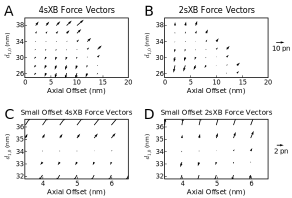
\includegraphics[width=3.2in]{../imgs/Figure4.pdf}
    \label{fig:force}
    \caption{
        \textbf{Force vectors of the two and four spring crossbridges, and the differences between.}        
    }
    \end{center}
\end{figure}

\begin{figure}[htbp]
    \begin{center}
    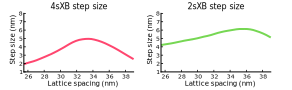
\includegraphics[width=3.2in]{../imgs/FigureS1.pdf}
    \label{fig:one_spring_comparison}
    \caption{
        Comparison of traditional single spring crossbridge properties to those of the two spring crossbridge at resting lattice spacing.}
    \end{center}
\end{figure}

\begin{figure}[htbp]
    \begin{center}
    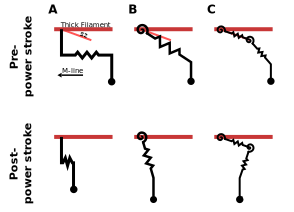
\includegraphics[width=3.2in]{../imgs/FigureS2.pdf}
    \label{fig:force_components}
    \caption{
        Separated axial and radial components of force exerted by the two spring crossbridge at several lattice spacings.}
    \end{center}
\end{figure}

% section figures (end)



% bibliography (fold)
% Bib style requires biophysj.bst be in the document directory
\clearpage
\bibliographystyle{biophysj}
\bibliography{SingleXB}
% bibliography (end)

\end{document}
